\documentclass[11pt,a4paper]{article}

\usepackage[margin=0.9in]{geometry}
\usepackage{graphicx}
\usepackage{booktabs}
\usepackage{amsmath}
\usepackage{hyperref}
\usepackage{float}
\usepackage{caption}
\usepackage[T1]{fontenc}
\usepackage{lmodern}
\usepackage{microtype}
\usepackage{enumitem}

\captionsetup{font=small,skip=4pt}
\setlength{\parskip}{3pt plus 1pt}
\setlength{\parindent}{1em}
\setlist{nosep,leftmargin=1.2em}

\graphicspath{{../data/analysis/}}

\title{Plurality Collapse: Measuring the Dimensionality Gap\\Between Human and LLM Moral Reasoning\\[0.3em]\large Milestone 2 Report}
\author{Xan Carey}
\date{April 2026}

\begin{document}
\maketitle
\vspace{-1em}

%% ============================================================================
\section{Methodology}
%% ============================================================================

\subsection{Dataset and Embedding}

We draw on the Sachdeva et al.\ dataset of 10,826 moral dilemmas from Reddit's ``Am I the Asshole'' forum. Each dilemma includes a top human comment alongside rationales from seven LLMs (GPT-3.5, GPT-4, Claude, Bison, Gemma, Mistral, Llama), each providing 2--3 rationales per dilemma for 216,497 LLM rationales total.

All rationales are encoded with Kaleido-XL, an encoder-decoder model trained on ValuePrism (31K moral situations with value annotations). Mean-pooling the encoder's final hidden states yields a 2048-dimensional embedding per rationale. Because Kaleido's space is organized around moral knowledge, geometric dimensionality serves as a proxy for reasoning diversity. We replicate all core analyses with Sentence-BERT (\texttt{all-mpnet-base-v2}, 768-dim) to control for encoder-specific bias.

\subsection{Analysis Pipeline}

Our analysis has four stages. First, we measure dimensionality via PCA, computing the participation ratio $\text{PR} = (\sum \lambda_i)^2 / \sum \lambda_i^2$ (effective variance-carrying dimensions) and comp90 (components for 90\% cumulative variance, sensitive to the eigenvalue tail). Robustness checks include matched-$n$ subsampling (5 seeds), dilemma-matched subsampling, word-count-quintile binning, and kernel PCA (RBF).

Second, we test for asymmetry by projecting each source's data onto the other's principal components and comparing variance captured in each direction.

Third, we qualify what the cross-projection residuals contain. Kaleido's decoder generates a moral value label per rationale; we collapse the 324 unique labels into semantic clusters (Sentence-BERT + $k$-means) and correlate residual magnitude with value diversity in sliding windows ($w{=}200$, step${=}50$) along the reconstruction error axis.

Fourth, we measure local LLM density around each human rationale via $k$-nearest neighbors ($k{=}50$) in PCA-reduced space, correlating density with reconstruction errors.

%% ============================================================================
\section{Results}
%% ============================================================================

\subsection{Dimensionality Gap}

Human rationales require 448 PCA components for 90\% variance, compared to 329--341 for individual LLMs and 347 for the pooled all-LLM set (Table~\ref{tab:summary}). The cumulative variance curves in Figure~\ref{fig:cumvar} make this visible: human variance accumulates more slowly, with a longer tail past the point where LLM curves flatten.

\begin{table}[H]
\centering\small
\caption{PCA dimensionality per source (Kaleido-XL).}
\label{tab:summary}
\vspace{-0.5em}
\begin{tabular}{lrrrr}
\toprule
Source & $n$ & PR & Comp.\ 90\% & Comp.\ 95\% \\
\midrule
Human   & 10,826  & 52.40 & 448 & 785 \\
GPT-3.5 & 32,478  & 49.76 & 329 & 642 \\
GPT-4   & 21,652  & 54.36 & 341 & 658 \\
Claude  & 32,478  & 52.06 & 340 & 653 \\
Bison   & 32,478  & 52.00 & 336 & 652 \\
Gemma   & 32,478  & 46.16 & 334 & 653 \\
Mistral & 32,455  & 42.65 & 332 & 654 \\
Llama   & 32,478  & 51.08 & 333 & 651 \\
All LLM & 216,497 & 51.95 & 347 & 679 \\
\bottomrule
\end{tabular}
\end{table}

\vspace{-0.5em}
\begin{figure}[H]
\centering
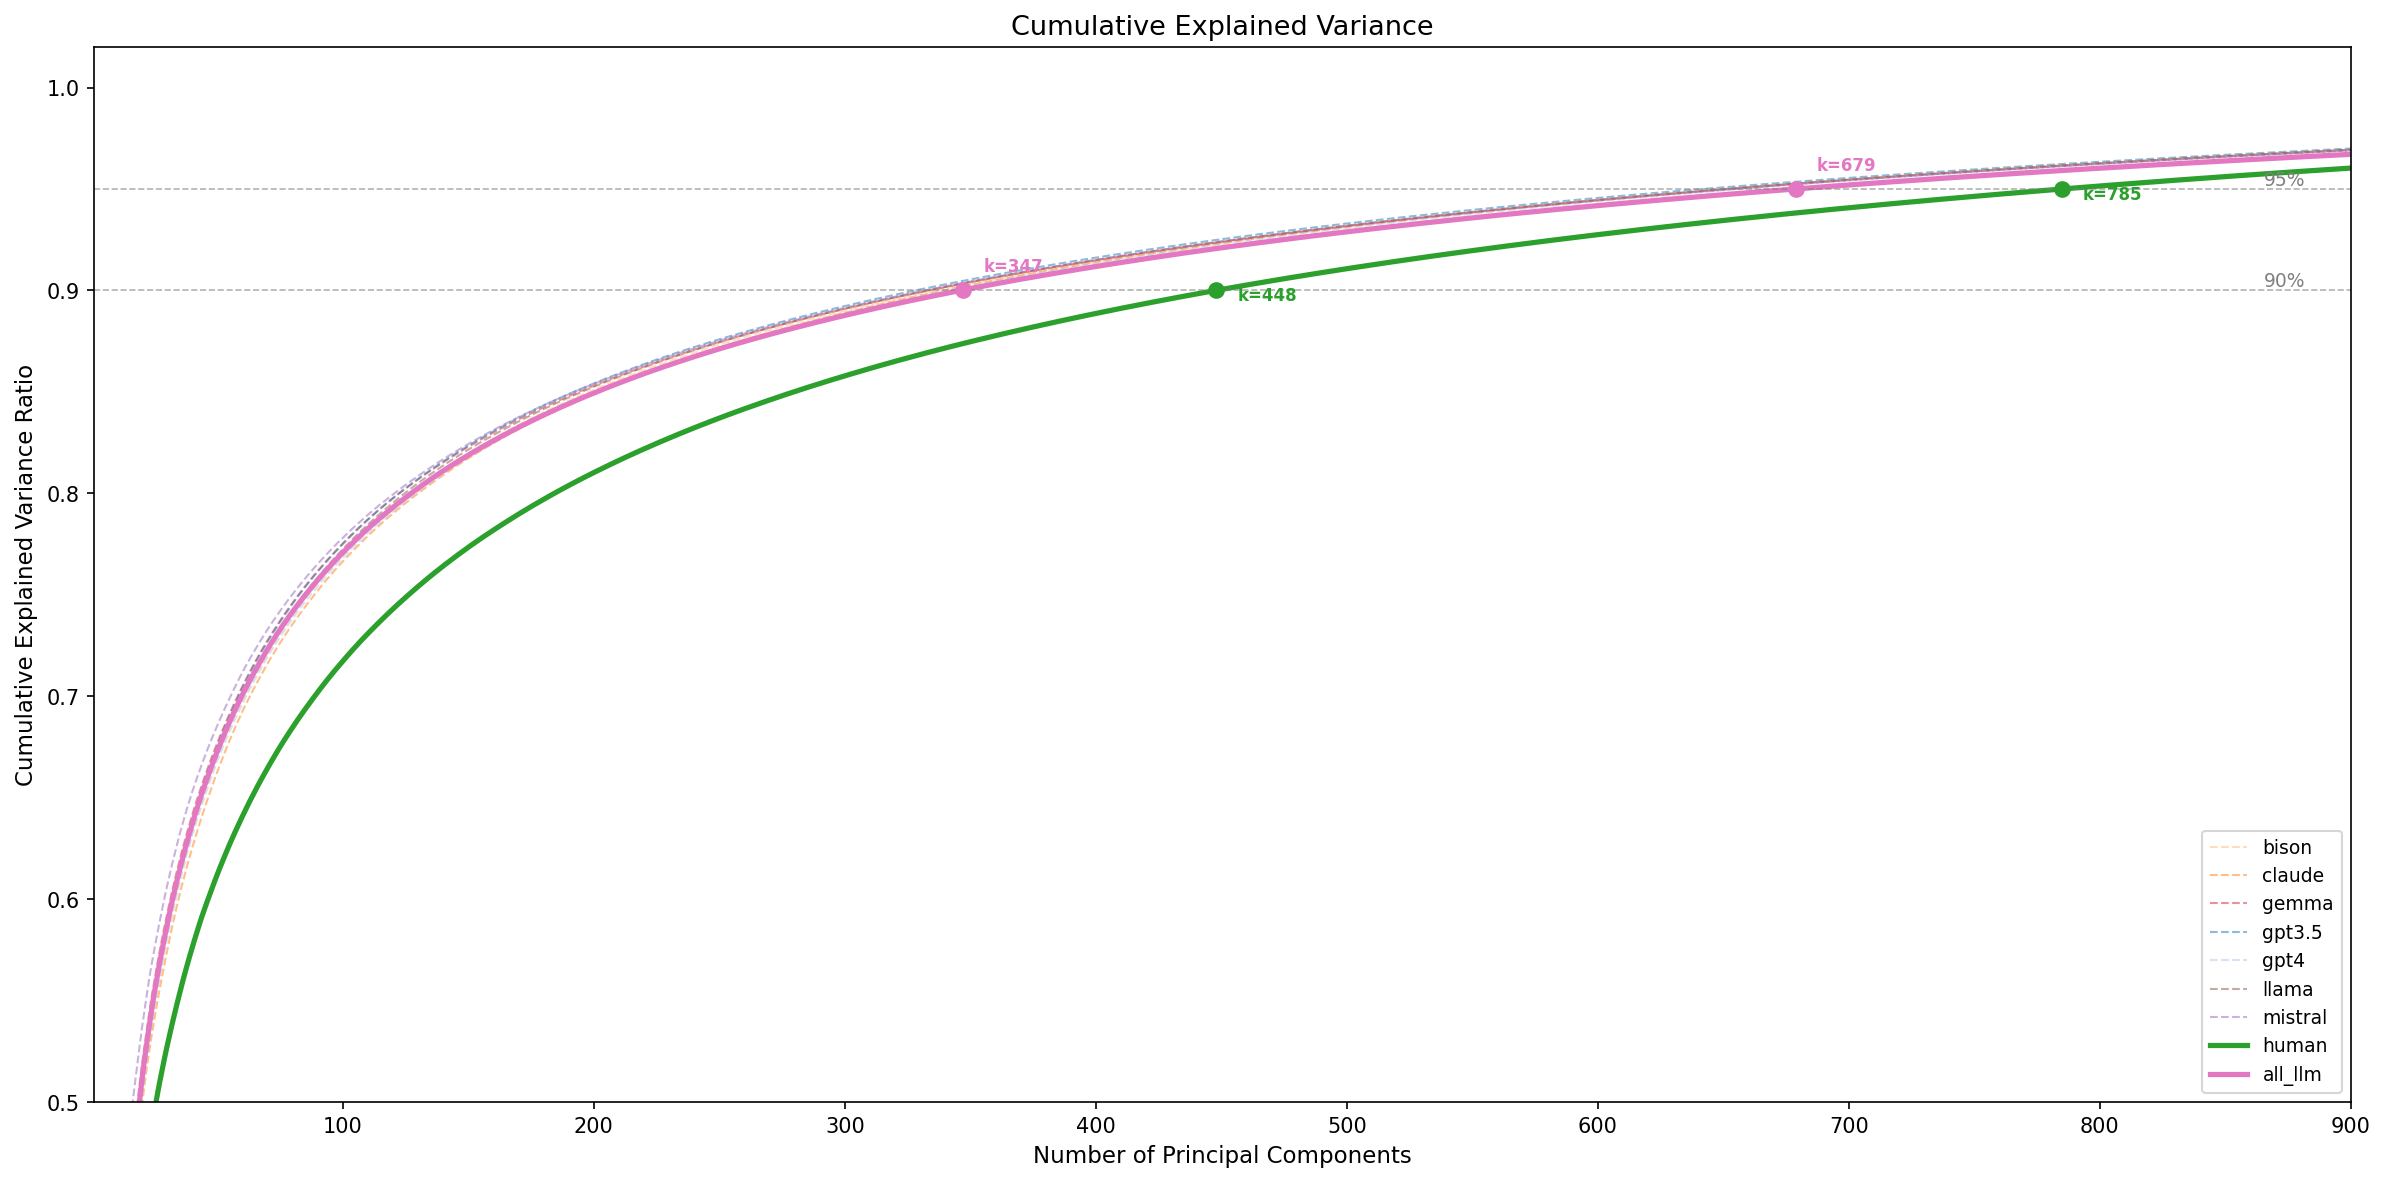
\includegraphics[width=0.82\textwidth]{cumulative_variance.png}
\vspace{-0.5em}
\caption{Cumulative explained variance by PCA components. Human reaches 90\% at $k{=}448$; all-LLM at $k{=}347$.}
\label{fig:cumvar}
\end{figure}

When we subsample each LLM to $n{=}10{,}826$ to match the human count, the gap is 35--41\%: LLMs need only 317--332 components. Dilemma-matched subsampling (picking exactly 1 of each LLM's 2--3 rationales per dilemma) shifts comp90 by only 2--5 components. The gap also persists across all word-count quintiles (30--47\% per bin), and kernel PCA yields near-identical PR rankings ($r = 0.984$), ruling out nonlinear structure.

\subsection{Asymmetric Overlap}

Cross-projection reveals a directional gap. Human PCs ($k{=}448$) capture 87.3\% of all-LLM variance, while all-LLM PCs ($k{=}347$) capture only 81.6\% of human variance---a 5.7pp asymmetry (Figure~\ref{fig:heatmap}). LLM reasoning largely lives within the human subspace, but not vice versa. Per-model: LLM PCs capture 77.5--81.3\% of human variance; human PCs capture 85.8--87.7\% of each LLM. SBERT shows an even wider asymmetry of 9.4pp.

\begin{figure}[H]
\centering
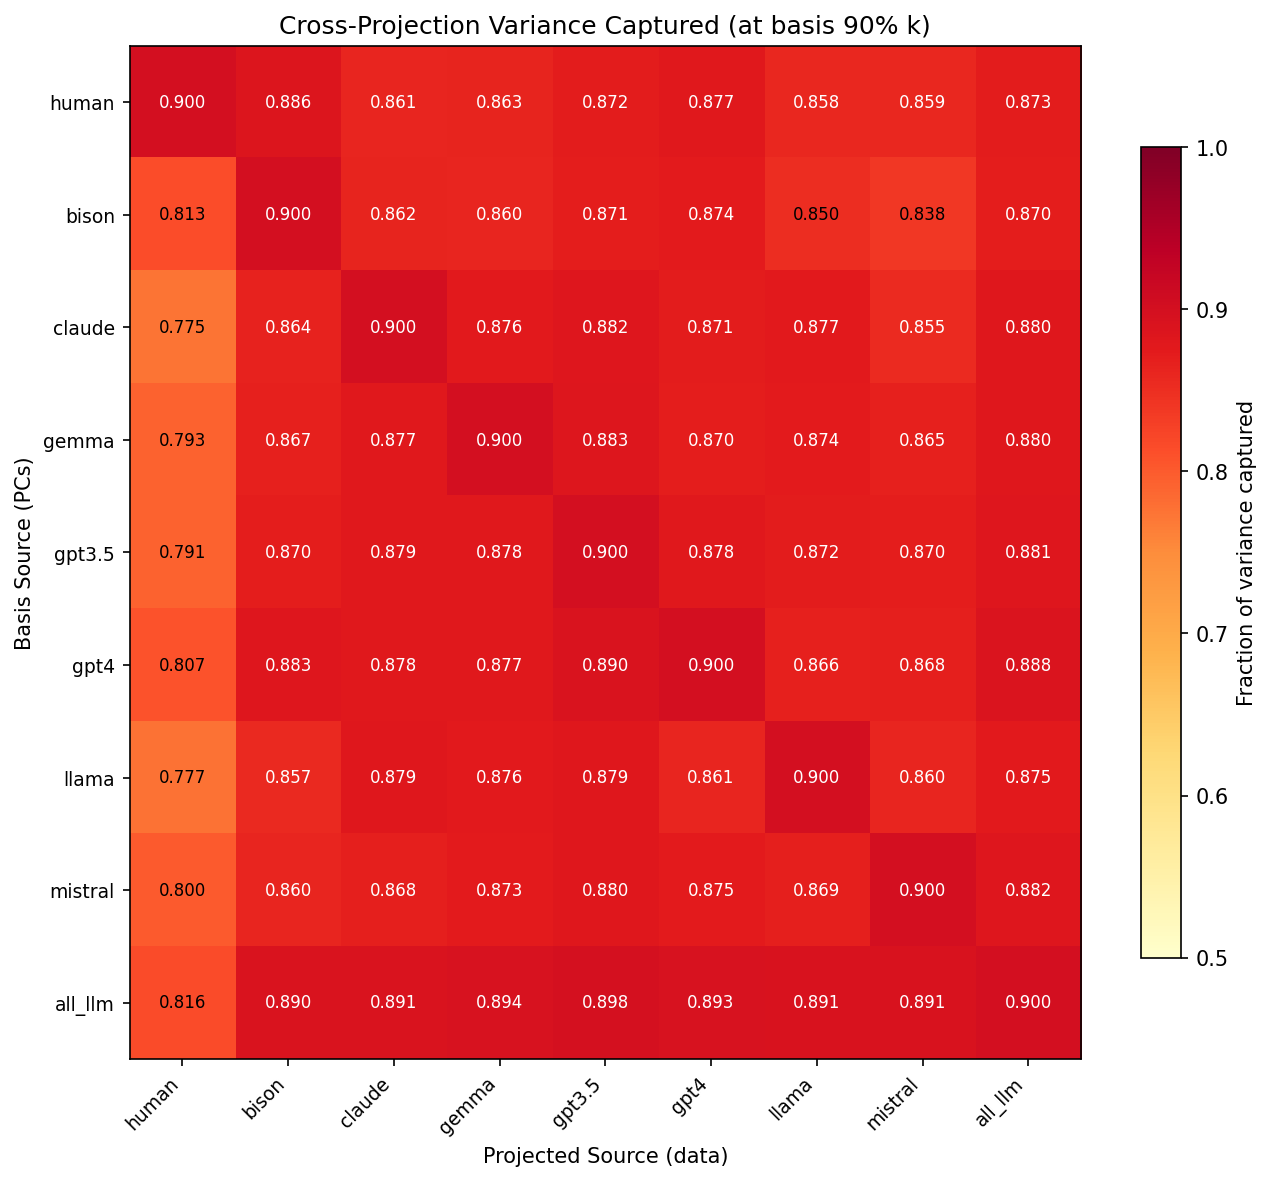
\includegraphics[width=0.62\textwidth]{cross_projection_heatmap.png}
\vspace{-0.5em}
\caption{Cross-projection heatmap. Human-basis$\to$LLM values (top row) systematically exceed LLM-basis$\to$human values (left column).}
\label{fig:heatmap}
\end{figure}

\subsection{Moral Content in the Extra Dimensions}

Do the extra human dimensions reflect moral content or just stylistic noise? We use Kaleido's decoder to generate a value label for each rationale, sort by reconstruction error under LLM PCs, and bin with a sliding window. The correlation between error and unique value clusters is $r = 0.897$ ($p < 0.0001$, Figure~\ref{fig:gradient}): rationales that LLM PCs fail to capture invoke more diverse moral values. The reverse direction yields $r = 0.823$. TF-IDF does turn up some stylistic markers among high-residual rationales, but the gradient is measured through decoded value labels, independent of surface text.

\begin{figure}[H]
\centering
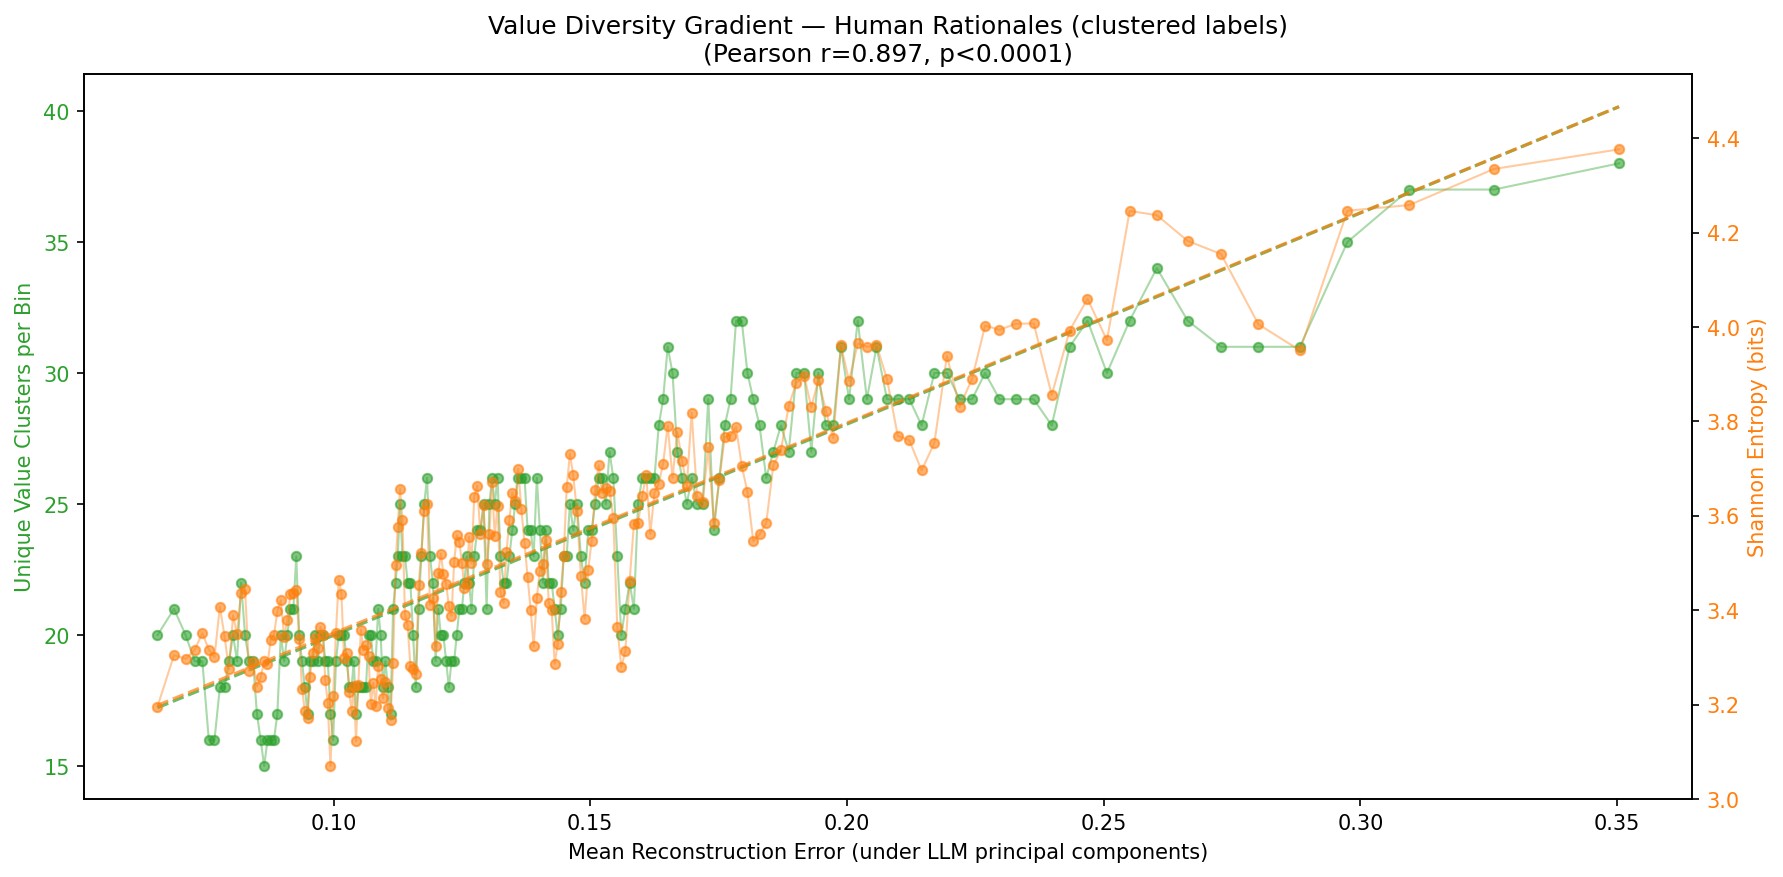
\includegraphics[width=0.82\textwidth]{value_diversity_sliding.png}
\vspace{-0.5em}
\caption{Value diversity gradient (sliding window, $w{=}200$). Unique clusters and entropy both rise with reconstruction error.}
\label{fig:gradient}
\end{figure}

\subsection{Frequency Compression}

Does the gap represent regions LLMs never visit, or regions they visit less often? KNN analysis shows the latter. Mean distance to 50 nearest LLM neighbors correlates with reconstruction error at $r = 0.969$ (binned) and $r = 0.846$ (per-rationale); the density ratio reaches $r = 0.988$ binned. LLMs span most of the space but concentrate mass in a smaller region, visiting the moral periphery less frequently than humans.

%% ============================================================================
\section{Analysis}
%% ============================================================================

Across the four stages, the picture is consistent: human moral reasoning occupies a higher-dimensional subspace, the gap is asymmetric, the extra dimensions carry moral content, and the mechanism is frequency compression rather than categorical absence.

We tested and ruled out four confounds. The gap survives matched-$n$ subsampling with less than 1 component of seed variation against a 114--131 component gap. It persists within every word-count quintile. Kernel PCA produces near-identical rankings ($r = 0.984$), ruling out nonlinear structure. And Sentence-BERT---which has never seen GPT-4 moral training data---replicates the gap with proportionally similar magnitude, with the cross-projection asymmetry actually larger in SBERT (9.4\% vs.\ 5.7\%).

The value diversity gradient ($r = 0.897$) links the extra dimensions to moral content: rationales that LLM PCs fail to reconstruct invoke the most diverse moral values. Combined with the KNN density results, this suggests LLMs are not missing moral categories entirely but under-representing the periphery of the value distribution.

The analysis does rely on a single dataset (Reddit AITA), and Kaleido's decoder was trained on GPT-4-generated labels, creating a potential circularity when qualifying one LLM source's residuals. SBERT addresses encoder bias but not this decoder dependency. The seven LLMs also represent a particular generation of models.

%% ============================================================================
\section{Plan for Additional Analysis}
%% ============================================================================

Several extensions would strengthen or clarify these findings.

We plan to stratify dilemmas by community consensus (low $<0.5$, medium $0.5$--$0.8$, high $>0.8$ agreement) and test whether the gap varies with moral controversy. If LLMs flatten diversity uniformly regardless of how contested a dilemma is, that points to a structural rather than context-dependent bias. Bootstrap resampling at matched $n$ will control for unequal bin sizes.

We also want to test whether $k$-means clustering on the rationale embeddings produces meaningful discrete structure (via silhouette scores and gap statistics), comparing joint vs.\ per-source clustering. Near-zero silhouette scores would confirm that the moral value space is better understood as a continuum, validating our geometric approach over categorical methods used in prior work.

On the model side, all seven LLMs show similar comp90 values (329--341), but their residual profiles may differ. Per-model cross-projection residuals mapped to specific value categories could reveal whether the compression is a shared training artifact or model-specific.

Finally, if plurality collapse is a frequency bias rather than a capability limitation, targeted prompting may help recover diversity. We plan to test persona-based prompts, explicit diversity instructions, and chain-of-thought with moral framework enumeration, measuring whether any strategy shifts LLM distributions toward higher dimensionality.

\end{document}
